\documentclass[11pt, a4paper]{article}
\usepackage[utf8]{inputenc}
\usepackage{amsmath,setspace,geometry}
\usepackage{amsthm}
\usepackage{amsfonts}
\usepackage[shortlabels]{enumitem}
\usepackage{rotating}
\usepackage{pdflscape}
\usepackage{graphicx}
\usepackage{bbm}
\usepackage[dvipsnames]{xcolor}
\usepackage{hyperref}
\hypersetup{colorlinks=true, linkcolor= BrickRed, citecolor = BrickRed, filecolor = BrickRed, urlcolor = BrickRed, hypertexnames = true}
\usepackage[]{natbib} 
\bibpunct[:]{(}{)}{,}{a}{}{,}
\geometry{left = 1.0in,right = 1.0in,top = 1.0in,bottom = 1.0in}
\usepackage[english]{babel}
\usepackage{float}
\usepackage{caption}
\usepackage{subcaption}
\usepackage{booktabs}
\usepackage{pdfpages}
\usepackage{threeparttable}
\usepackage{lscape}
\usepackage{bm}
\setstretch{1.4}
%\usepackage[tablesfirst,nolists]{endfloat}

\newtheorem{theorem}{Theorem}
\newtheorem{assumption}{Assumption}
\newtheorem{lemma}{Lemma}
\newtheorem{definition}{Definition}
\newtheorem{proposition}{Proposition}
\newtheorem{claim}{Claim}
\newtheorem{corollary}{Corollary}
\newtheorem{example}{Example}
\DeclareMathOperator{\rank}{rank}


\title{Finite Sample Performance of a Conduct Parameter Test in Homogenous Goods Markets}
\author{Yuri Matsumura\thanks{Department of Economics, Rice University. Email: Yuri.Matsumura@rice.edu} \and Suguru Otani \thanks{Department of Economics, Rice University. Email: so19@rice.edu
%Declarations of interest: none %this is for Economics Letters
}}

\begin{document}

\maketitle
\begin{abstract}
    We assess the finite sample performance of the conduct parameter test in homogeneous goods markets. Statistical power rises with an increase in the number of markets, a larger conduct parameter, and a stronger demand rotation instrument. However, even with a moderate number of markets and five firms, regardless of instrument strength and the utilization of optimal instruments, rejecting the null hypothesis of perfect competition remains challenging. Our findings indicate that empirical results that fail to reject perfect competition are a consequence of the limited number of markets rather than methodological deficiencies.
\vspace{0.1in}

\noindent\textbf{Keywords:} Conduct parameters, Homogenous goods market, Monte Carlo simulation, Statistical power analysis
\vspace{0in}
\newline
\noindent\textbf{JEL Codes:} C5, C13, L1

\bigskip
\end{abstract}


\section{Introduction}
Measuring competitiveness is important in the empirical industrial organization literature.
A conduct parameter is considered to be a useful measure of competitiveness. 
However, the parameter cannot be directly measured from data because data generally lack information about marginal costs.
Therefore, researchers endeavor to learn conduct parameters.

Researchers estimate and test structural models to understand firm conduct in both homogeneous and differentiated good markets \citep{nevoIdentificationOligopolySolution1998, magnolfi2022comparison, duarte2023testing}. 
We focus on homogenous good markets. 
The conduct parameters for the linear model are identified by \citet{bresnahan1982oligopoly}, and \cite{matsumura2023resolving} resolve conflicts between \cite{bresnahan1982oligopoly} and \cite{perloff2012collinearity} vis-a-vis identification problems. 
Estimation accuracy may be improved by adding equilibrium existence conditions in the log-linear model \citep{matsumura2023mpec}. 
Conduct parameter testing is undertaken by \cite{genesove1998testing}, who compare estimates from the sugar industry with direct measures of market power.\footnote{\cite{genesove1998testing} made mistakes on how to get predicted interaction terms of rotation demand instruments and endogenous quantity in the first stage regression. See Section A.3, \cite{matsumura2023resolving}.} 
When market power is around 0.1 and the number of markets is less than 100, perfect competition cannot be rejected. 
\cite{steen1999testing} study 48 markets in the French salmon industry and \cite{shaffer1993test} studies 25 markets in the Canadian banking industry. 
They also cannot reject the null hypothesis that markets are perfectly competitive. 
Their results raise doubts about the methodology in itself \citep{shafferMarketPowerCompetition2017}.


While popular, there is a lack of formal Monte Carlo simulations for a conduct parameter test. 
Accordingly, we investigate the finite sample performance of the conduct parameter test in homogeneous goods markets. 
We analyze statistical power by varying the number of markets, firms, and strength of demand rotation instruments under the null hypothesis of perfect competition.

Our findings indicate that statistical power increases with more markets, a larger conduct parameter, and stronger demand rotation instruments. 
However, even with a moderate number of markets (e.g., 1000) and five firms, we cannot achieve an 80\% rejection frequency ($1-\beta=0.8$, where $\beta$ represents the probability of a Type II error), irrespective of instrument strength and the use of optimal instruments. While optimal instruments enhance rejection probability in large samples, they do not alter the core findings. 
This highlights the challenge of testing perfect competition, as recognized by \cite{genesove1998testing}, \cite{steen1999testing}, and \cite{shaffer1993test}, primarily stemming from the limited number of markets rather than methodological flaws.

Our results and code provide a valuable reference for applied researchers examining assumptions about firm conduct in homogeneous goods markets, i.e., whether it is perfect competition, Cournot competition, or perfect collusion.

\section{Model}
Consider data with $T$ markets with homogeneous products.
Assume that there are $N$ firms in each market.
Let $t = 1,\ldots, T$ be the index for markets.
Then, we obtain a supply equation:
\begin{align}
     P_{t} = -\theta\frac{\partial P_{t}(Q_{t})}{\partial Q_{t}}Q_{t} + MC_{t}(Q_{t}),\label{eq:supply_equation}
\end{align}
where $Q_{t}$ is the aggregate quantity, $P_{t}(Q_{t})$ is the demand function, $TC_{t}(Q_{t})$ is the marginal cost function, and $\theta\in[0,1]$ is  the conduct parameter. 
The equation nests perfect competition ($\theta=0$), Cournot competition ($\theta=1/N$), and perfect collusion ($\theta=1$) (See \cite{bresnahan1982oligopoly}). 

Consider an econometric model that integrates the above.
Assume that the demand and marginal cost functions are written as: 
\begin{align}
    P_{t} = f(Q_{t}, Y_{t}, \varepsilon^{d}_{t}, \alpha), \label{eq:demand}\\
    MC_{t} = g(Q_{t}, W_{t}, \varepsilon^{c}_{t}, \gamma),\label{eq:marginal_cost}
\end{align}
where $Y_{t}$ and $W_{t}$ are vectors of exogenous variables, $\varepsilon^{d}_{t}$ and $\varepsilon^{c}_{t}$ are error terms, and $\alpha$ and $\gamma$ are vectors of parameters.
Additionally, we have demand- and supply-side instruments, $Z^{d}_{t}$ and $Z^{c}_{t}$, and assume that the error terms satisfy the mean independence conditions, $E[\varepsilon^{d}_{t}\mid Y_{t}, Z^{d}_{t}] = E[\varepsilon^{c}_{t} \mid W_{t}, Z^{c}_{t}] =0$.

\subsection{Linear demand and cost}
Assume that linear demand and marginal cost functions are specified as:
\begin{align}
    P_{t} &= \alpha_0 - (\alpha_1 + \alpha_2Z^{R}_{t})Q_{t} + \alpha_3 Y_{t} + \varepsilon^{d}_{t},\label{eq:linear_demand}\\
    MC_{t} &= \gamma_0  + \gamma_1 Q_{t} + \gamma_2 W_{t} + \gamma_3 R_{t} + \varepsilon^{c}_{t},\label{eq:linear_{t}arginal_cost}
\end{align}
where $W_{t}$ and $R_{t}$ are exogenous cost shifters and $Z^{R}_{t}$ is Bresnahan's demand rotation instrument. 
The supply equation is written as:
\begin{align}
    P_{t} 
    %&= \gamma_0 + [\theta(\alpha_1 + \alpha_2Z^{R}_{t})+ \gamma_1] Q_{t}   + \gamma_2 W_{t} + \gamma_3 R_{t} + \varepsilon^{c}_{t}\nonumber\\ 
    &= \gamma_0 + \theta (\alpha_1 + \alpha_2 Z^{R}_{t})Q_{t} + \gamma_1 Q_{t} + \gamma_2 W_{t} + \gamma_3 R_{t} +\varepsilon^c_{t}.\label{eq:linear_supply_equation}\end{align}
By substituting Equation \eqref{eq:linear_demand} with Equation \eqref{eq:linear_supply_equation} and solving it for $P_{t}$, we obtain the aggregate quantity $Q_{t}$ based on the parameters and exogenous variables as follows:
\begin{align}
    Q_{t} =  \frac{\alpha_0 + \alpha_3 Y_{t} - \gamma_0 - \gamma_2 W_{t} - \gamma_3 R_{t} + \varepsilon^{d}_{t} - \varepsilon^{c}_{t}}{(1 + \theta) (\alpha_1 + \alpha_2 Z^{R}_{t}) + \gamma_1}.\label{eq:quantity_linear}
\end{align}


\section{Simulation results}\label{sec:results}

\subsection{Simulation and estimation procedure}

We set true parameters and distributions as shown in Table \ref{tb:parameter_setting}. 
We vary the true value of $\theta$ from 0.05 (20-firm symmetric Cournot) to 1 (perfect collusion) and the strength of demand rotation instrument, $\alpha_2$, from 0.1 (weak) to 20.0 (extremely strong) which is unrealistically larger than the price coefficient level, $\alpha_1=1.0$.
For simulation, we generate 100 datasets.
We separately estimate the demand and supply equations via two-stage least squares (2SLS) estimation.
The instrumental variables for demand estimation are $Z^{d}_{t} = (1, Z^{R}_{t}, Y_{t}, H_{t}, K_{t})$ and for supply estimation are $Z^{c}_{t} = (1, Z^{R}_{t}, W_{t}, R_{t}, Y_{t})$ for a benchmark model. 
To achieve theoretical efficiency bounds, we add optimal instruments of \cite{chamberlain1987asymptotic}, used in demand estimation \citep{reynaert2014improving}. 
Optimal instruments lead to asymptotically efficient estimators, as their asymptotic variance cannot be reduced via additional orthogonality conditions.
See Appendix \ref{sec:optimal_instruments} for construction details.
The null hypothesis is that markets are under perfect competition, that is, $\theta=0$.
We compute the rejection
frequency as the power by using t-statistics at a significance level of 0.05 over 100 datasets.

\begin{table}[!htbp]
    \caption{True parameters and distributions}
    \label{tb:parameter_setting}
    \begin{center}
    \subfloat[Parameters]{
    \begin{tabular}{cr}
            \hline
            $\alpha_0$ & $10.0$  \\
            $\alpha_1$ & $1.0$  \\
            $\alpha_2$ & $\{0.1,0.5,1.0,5.0,20.0\}$ \\
            $\alpha_3$ & $1.0$  \\
            $\gamma_0$ & $1.0$ \\
            $\gamma_1$ & $1.0$  \\
            $\gamma_2$ & $1.0$ \\
            $\gamma_3$ & $1.0$\\
            $\theta$ & $\{0.05,0.1,0.2,0.33,0.5,1.0\}$ \\
            \hline
        \end{tabular}
    }
    \subfloat[Distributions]{
    \begin{tabular}{crr}
            \hline
            Demand shifter&  \\
            $Y_{t}$ & $N(0,1)$  \\
            Demand rotation instrument&   \\
            $Z^{R}_{t}$ & $N(10,1)$ \\
            Cost shifter&    \\
            $W_{t}$ & $N(3,1)$  \\
            $R_{t}$ & $N(0,1)$   \\
            $H_{t}$ & $W_{t}+N(0,1)$  \\
            $K_{t}$ & $R_{t}+N(0,1)$   \\
            Error&  &  \\
            $\varepsilon^{d}_{t}$ & $N(0,\sigma)$  \\
            $\varepsilon^{c}_{t}$ & $N(0,\sigma)$ \\
            \hline
        \end{tabular}
    }
    \end{center}
    \footnotesize
    Note: $\sigma=1.0$. $N:$ Normal distribution. $U:$ Uniform distribution.
\end{table}

Figure \ref{fg:theta_hat_power} displays the finite sample performance results for the conduct parameter $\theta$.\footnote{Simulation details and additional results for all other parameters are available in the online appendix.} 
Rejection frequency increases under the following conditions: a large sample size (number of markets), a larger $\theta$ (fewer firms), and a larger $\alpha_2$ (stronger demand rotation instrument).
Panel (f) indicates that with 20 symmetric firms ($\theta=0.05$) and a sufficiently large number of markets, we achieve an approximately 70\% power to reject the null hypothesis of markets operating under perfect competition. 
However, we cannot reject the null hypothesis with an acceptable sample size and power when markets follow 20-firm symmetric Cournot competition.

A remarkable finding is that even with a moderate number of markets (e.g., 1000 in Panel (c)) and five firms, the rejection frequency cannot achieve 80\% (i.e., $1-\beta=0.8$, where $\beta$ is the probability of making a Type II error), regardless of instrument strength.
This implies that \cite{genesove1998testing}, using 97 markets, \cite{shaffer1993test}, using 25 markets, and \cite{steen1999testing}, using 48 markets, fail in rejecting perfect competition due to the small sample problem.

Figure \ref{fg:theta_hat_power_iv_optimal_relative_to_benchmark_10000} shows the efficiency gain of optimal instruments relative to the aforementioned benchmark model. 
We find that if the number of markets exceeds 1,000, optimal instruments increase the rejection probability. 
However, the gain does not change our benchmark results.


Why is it statistically challenging to differentiate between perfect and Cournot competition?
In differential product markets, as demonstrated by \citet{berry2014identification}, the variation in instrumental variables can aid in discerning firm behavior. 
Various factors such as changes in the number of products, prices in other markets, and alterations in product characteristics, can be utilized without requiring a specific functional form.
In contrast, homogeneous product markets exhibit limited variation only on demand rotation instruments. 
Therefore, even when the number of firms is substantial, firm conduct tests may lack the necessary power to differentiate between perfect and Cournot competition.

\begin{figure}[!ht]
  \begin{center}
  % \subfloat[M=50]{\includegraphics[width = 0.32\textwidth]
  % {figuretable/theta_hat_power_50.png}}
  \subfloat[$T=100$]{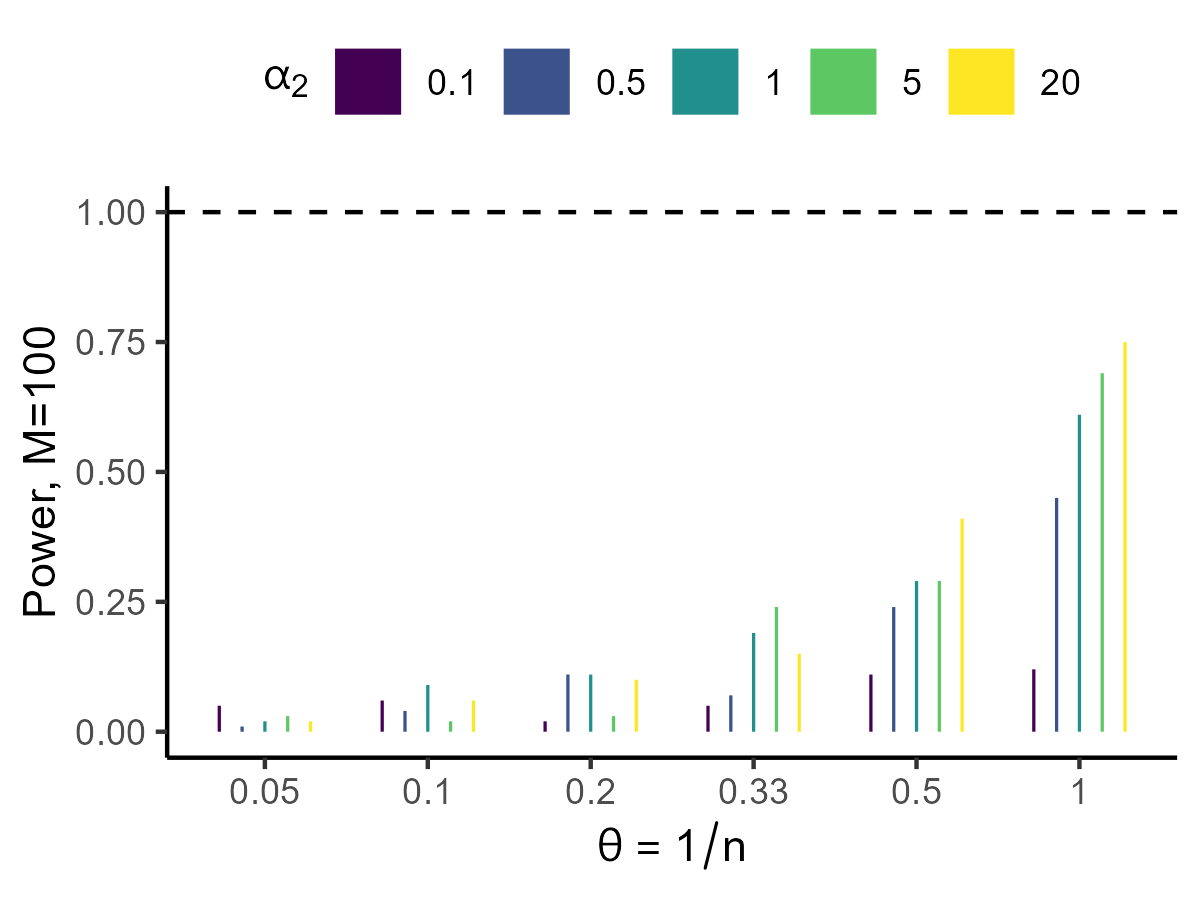
\includegraphics[width = 0.32\textwidth]
  {figuretable/theta_hat_power_100.png}}
  \subfloat[$T=200$]{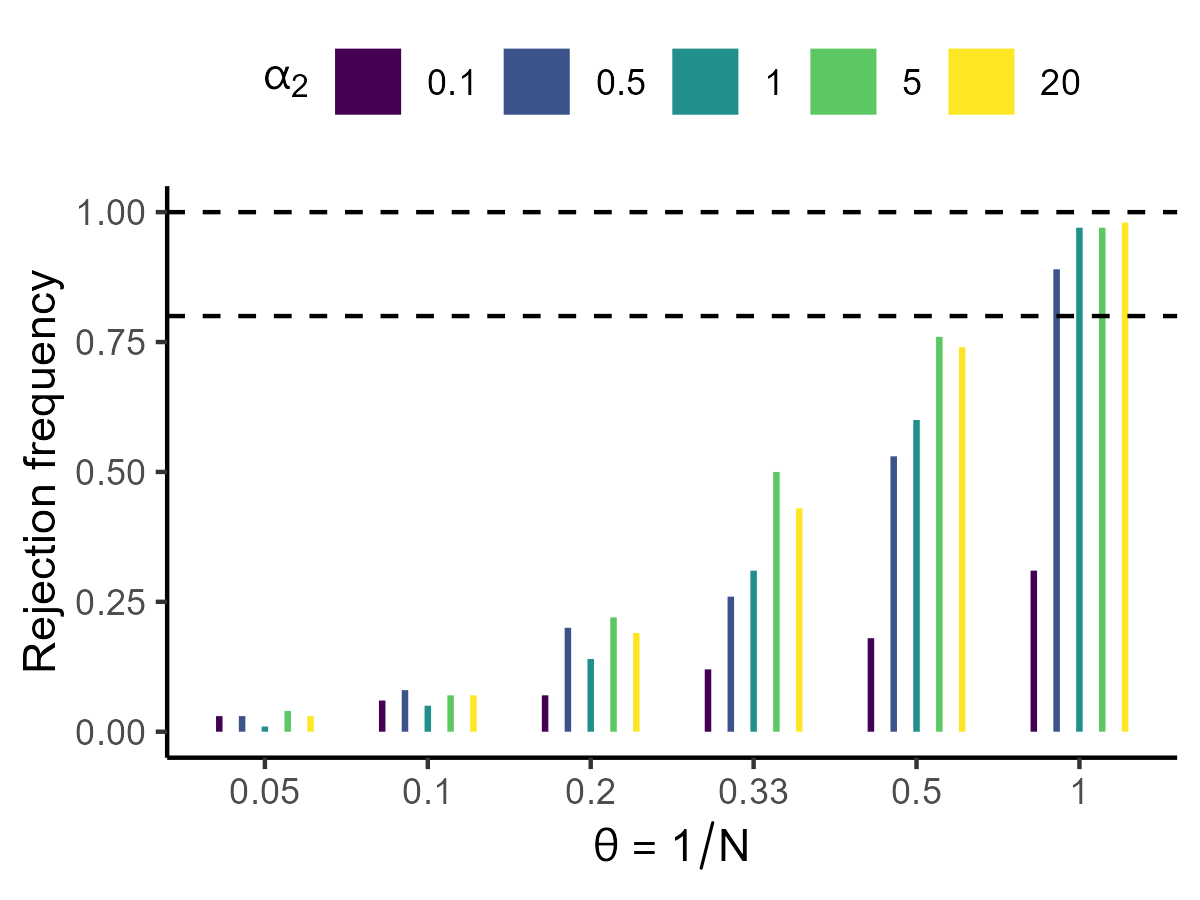
\includegraphics[width = 0.32\textwidth]
  {figuretable/theta_hat_power_200.png}}
  \subfloat[$T=1000$]{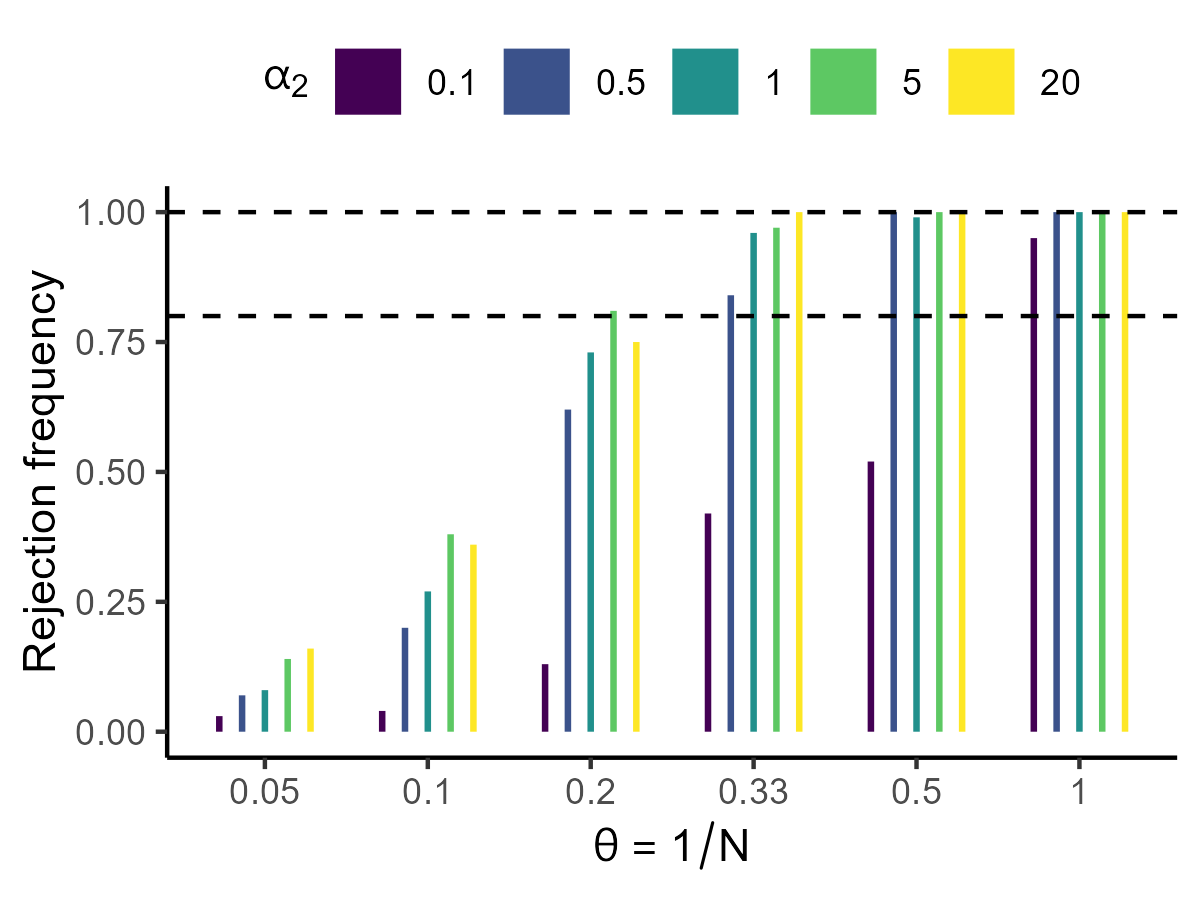
\includegraphics[width = 0.32\textwidth]
  {figuretable/theta_hat_power_1000.png}}\\
  \subfloat[$T=2000$]{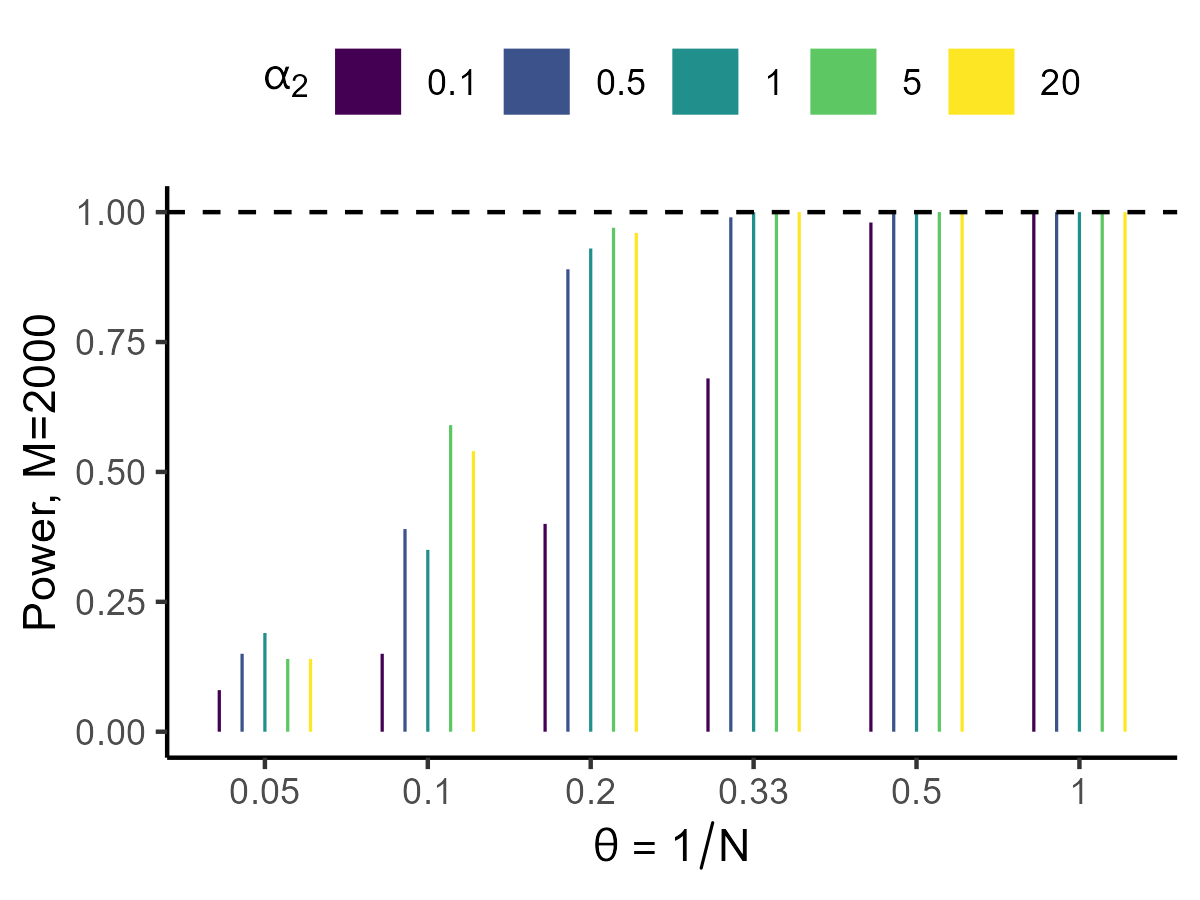
\includegraphics[width = 0.32\textwidth]
  {figuretable/theta_hat_power_2000.png}}
  \subfloat[$T=5000$]{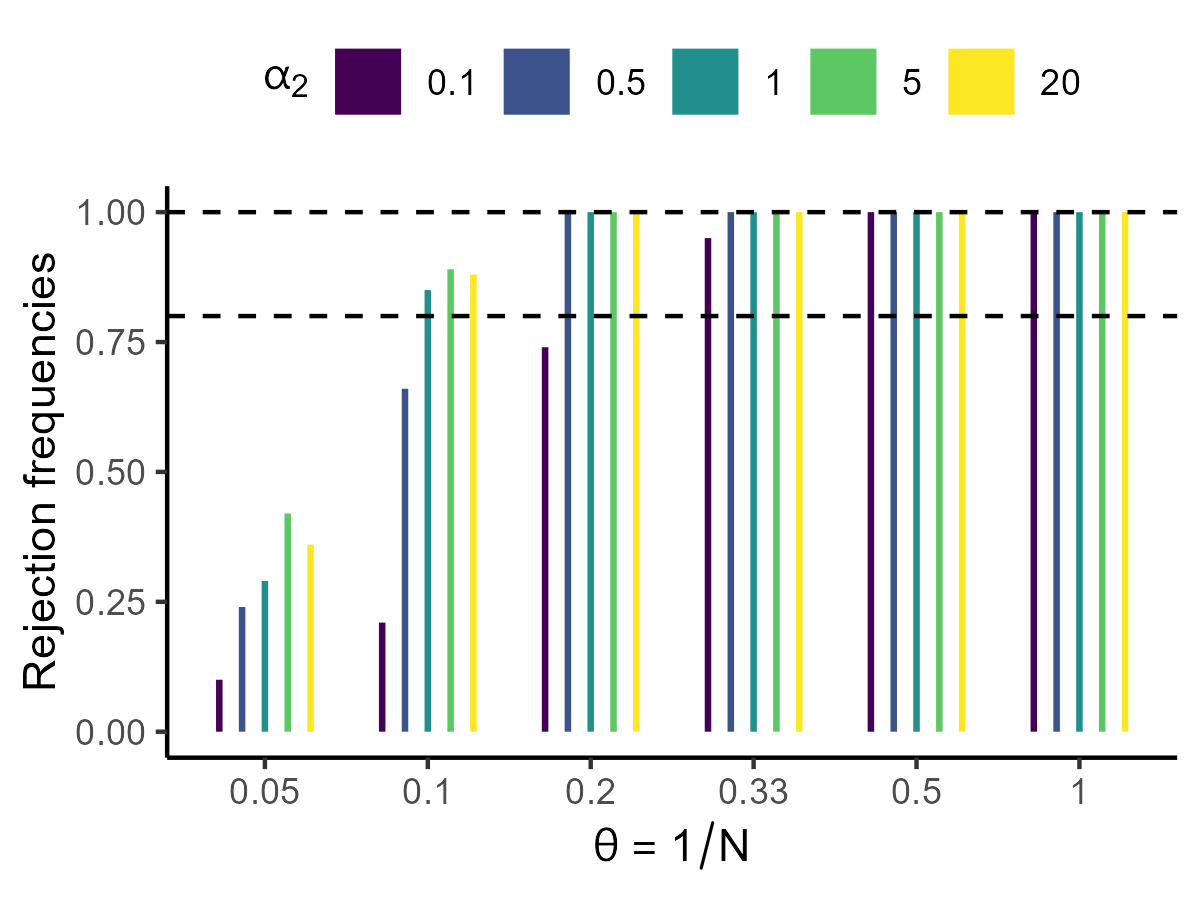
\includegraphics[width = 0.32\textwidth]
  {figuretable/theta_hat_power_5000.png}}
  \subfloat[$T=10000$]{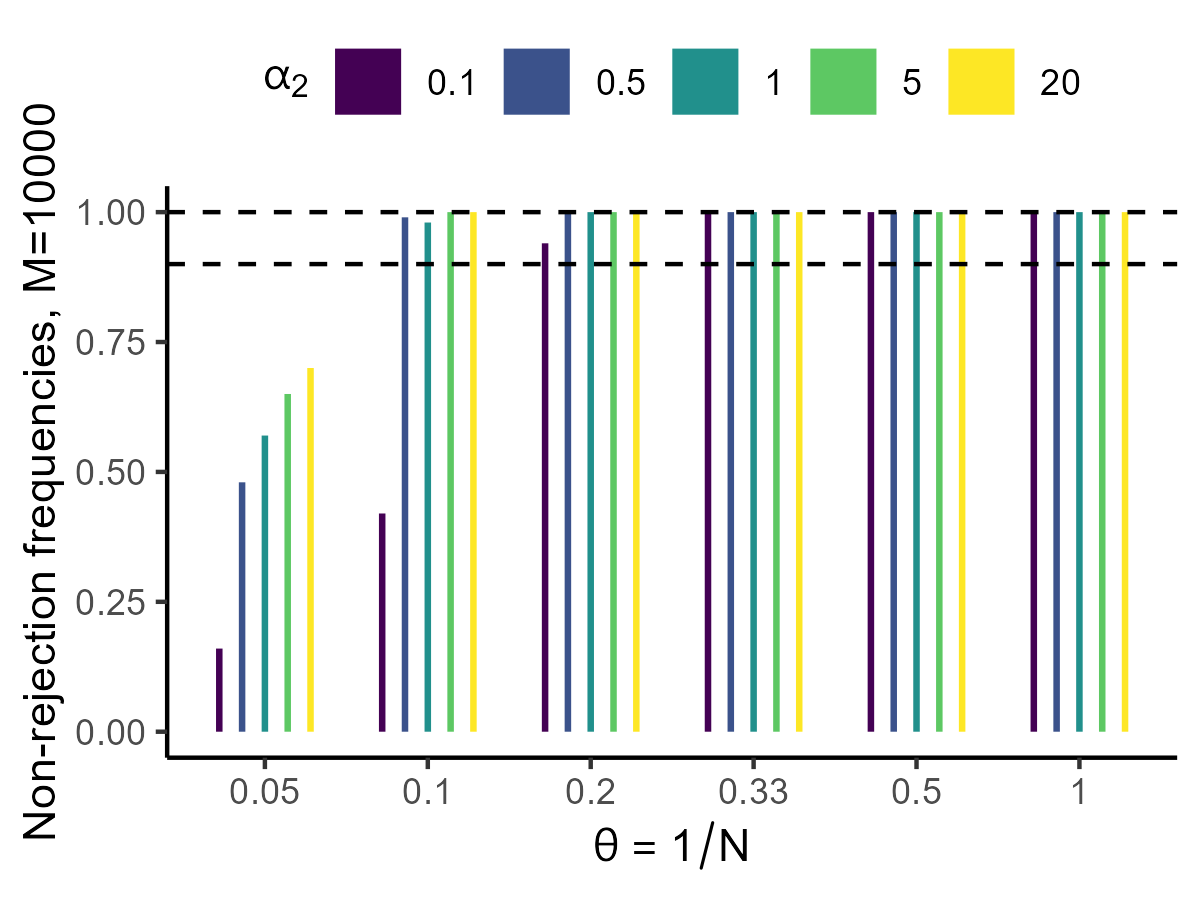
\includegraphics[width = 0.32\textwidth]
  {figuretable/theta_hat_power_10000.png}}
  \caption{Statistical power of conduct parameter $\theta$}
  \label{fg:theta_hat_power}
  \end{center}
  \footnotesize
  Note: Dotted lines are 80\% and 100\% rejection frequencies out of 100 simulation data.
\end{figure} 


\begin{figure}[!ht]
  \begin{center}
  % \subfloat[M=50]{\includegraphics[width = 0.32\textwidth]
  % {figuretable/theta_hat_power_50.png}}
  \subfloat[$T=100$]{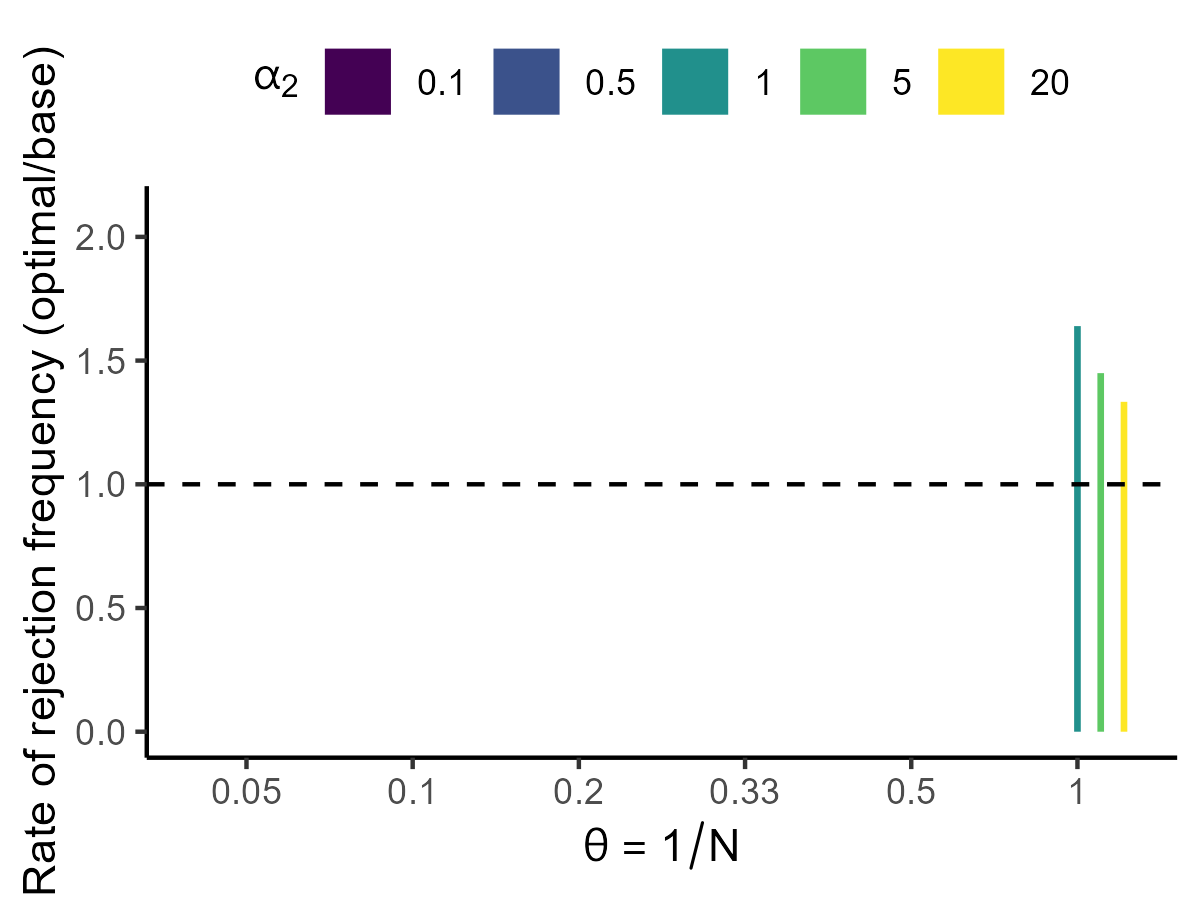
\includegraphics[width = 0.32\textwidth]
  {figuretable/theta_hat_power_iv_optimal_relative_to_benchmark_100.png}}
  \subfloat[$T=200$]{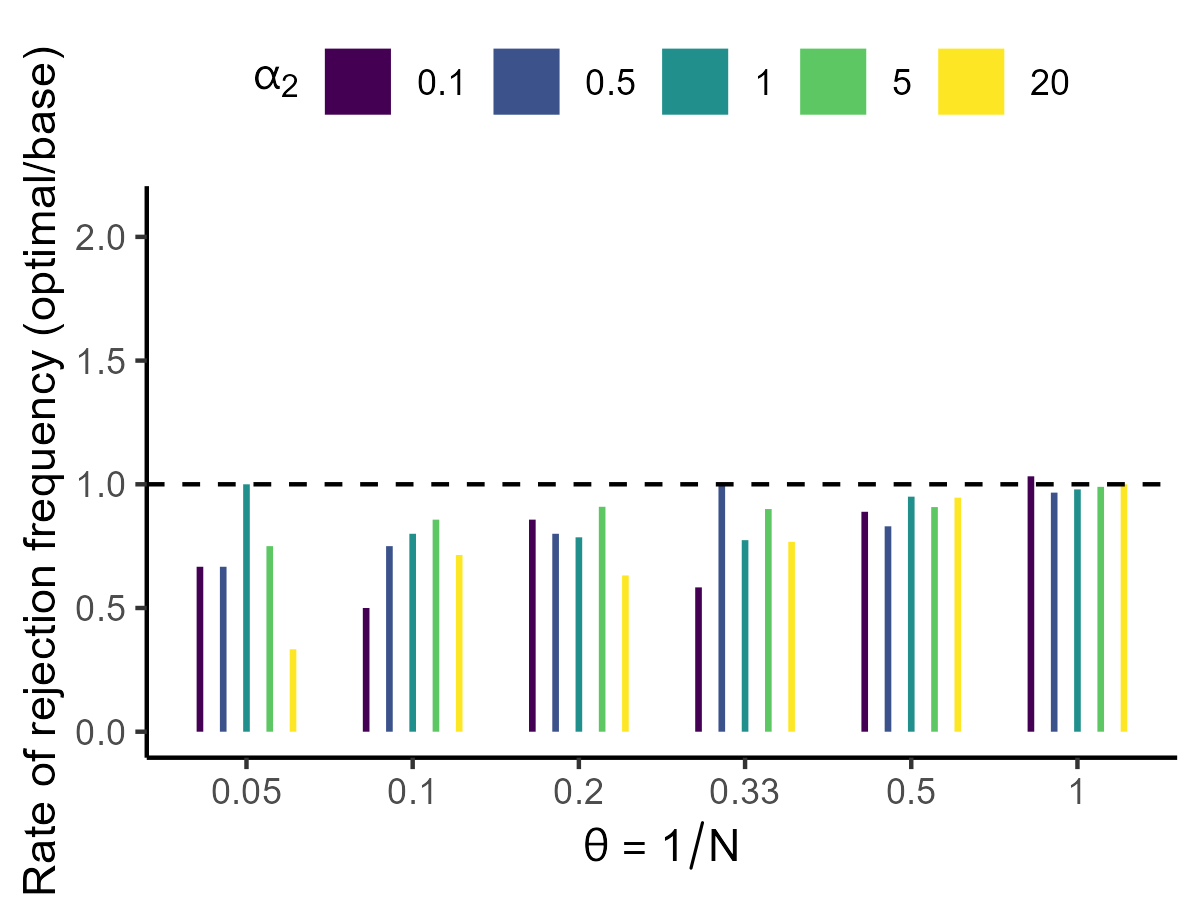
\includegraphics[width = 0.32\textwidth]
  {figuretable/theta_hat_power_iv_optimal_relative_to_benchmark_200.png}}
  \subfloat[$T=1000$]{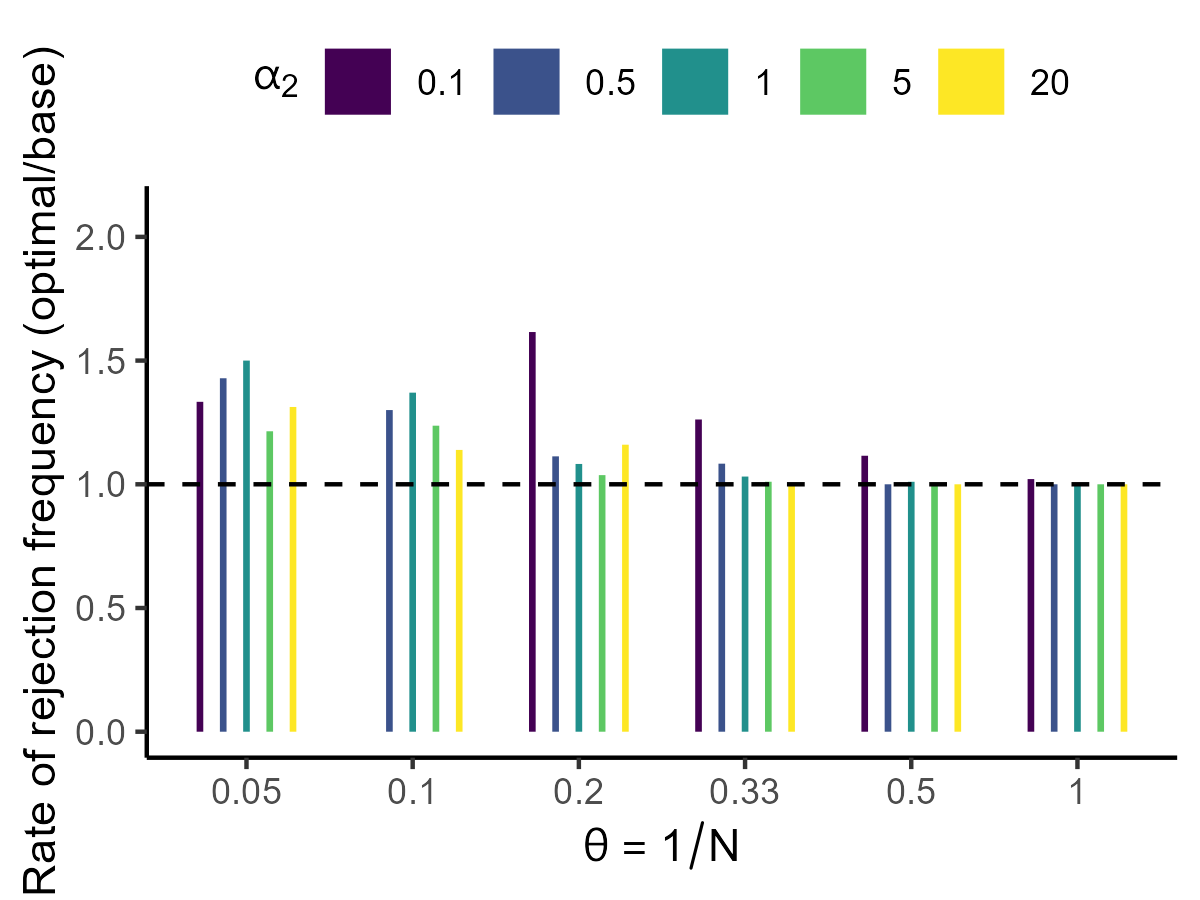
\includegraphics[width = 0.32\textwidth]
  {figuretable/theta_hat_power_iv_optimal_relative_to_benchmark_1000.png}}\\
  \subfloat[$T=2000$]{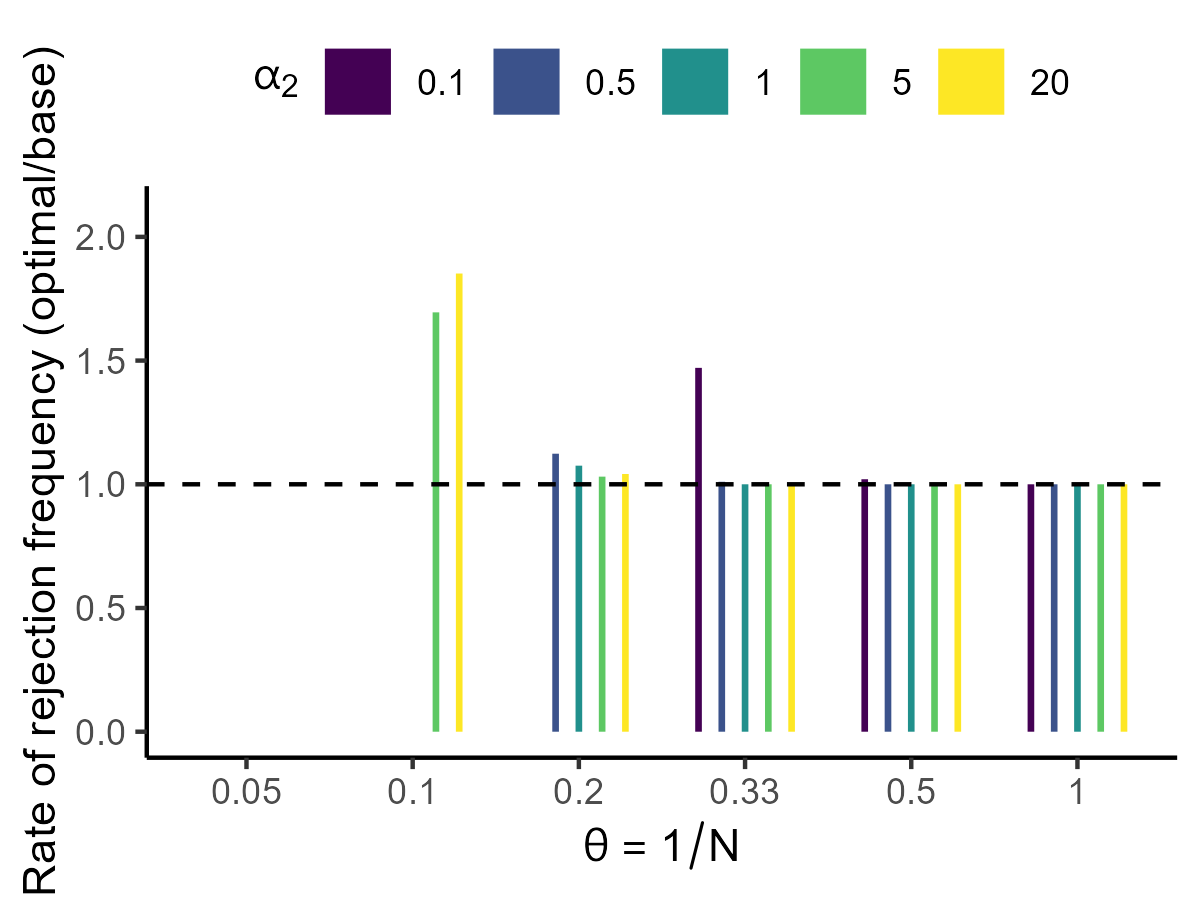
\includegraphics[width = 0.32\textwidth]
  {figuretable/theta_hat_power_iv_optimal_relative_to_benchmark_2000.png}}
  \subfloat[$T=5000$]{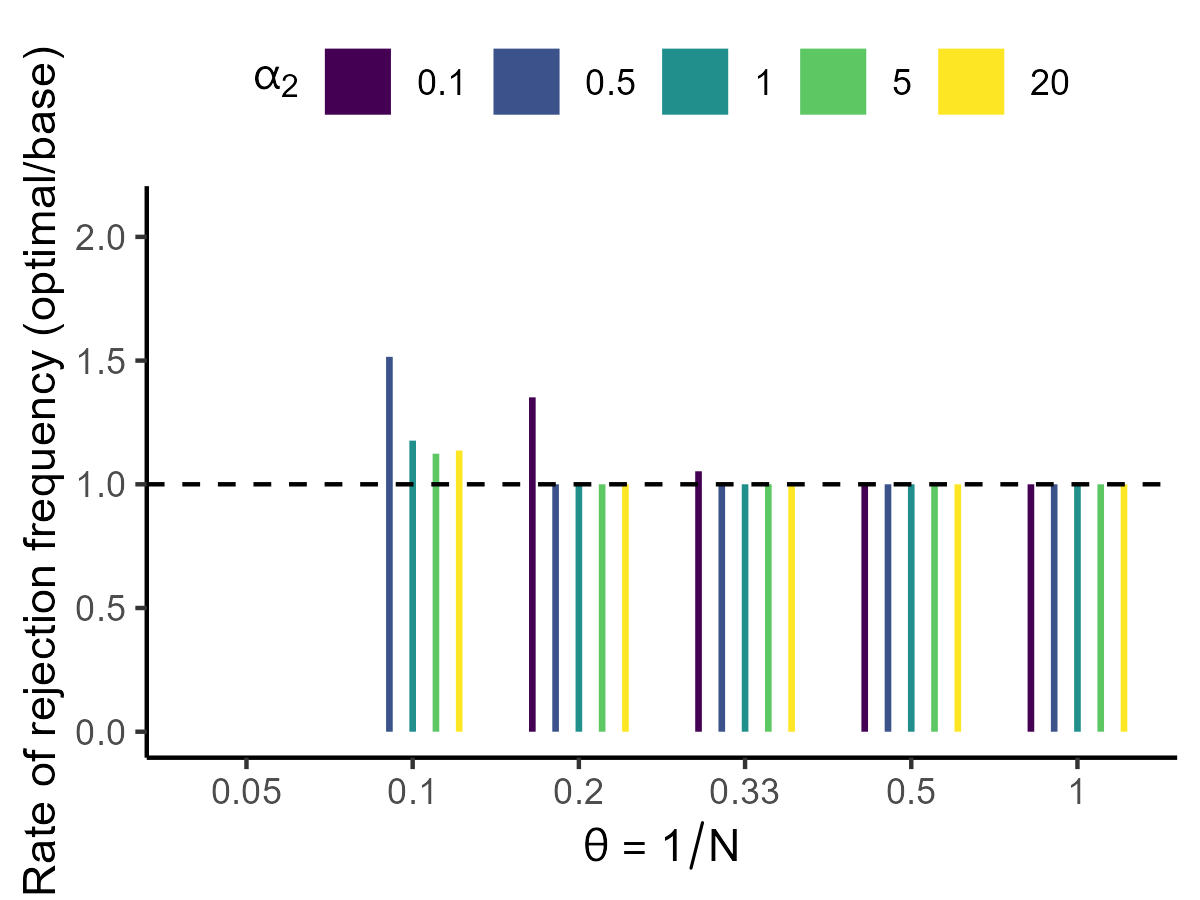
\includegraphics[width = 0.32\textwidth]
  {figuretable/theta_hat_power_iv_optimal_relative_to_benchmark_5000.png}}
  \subfloat[$T=10000$]{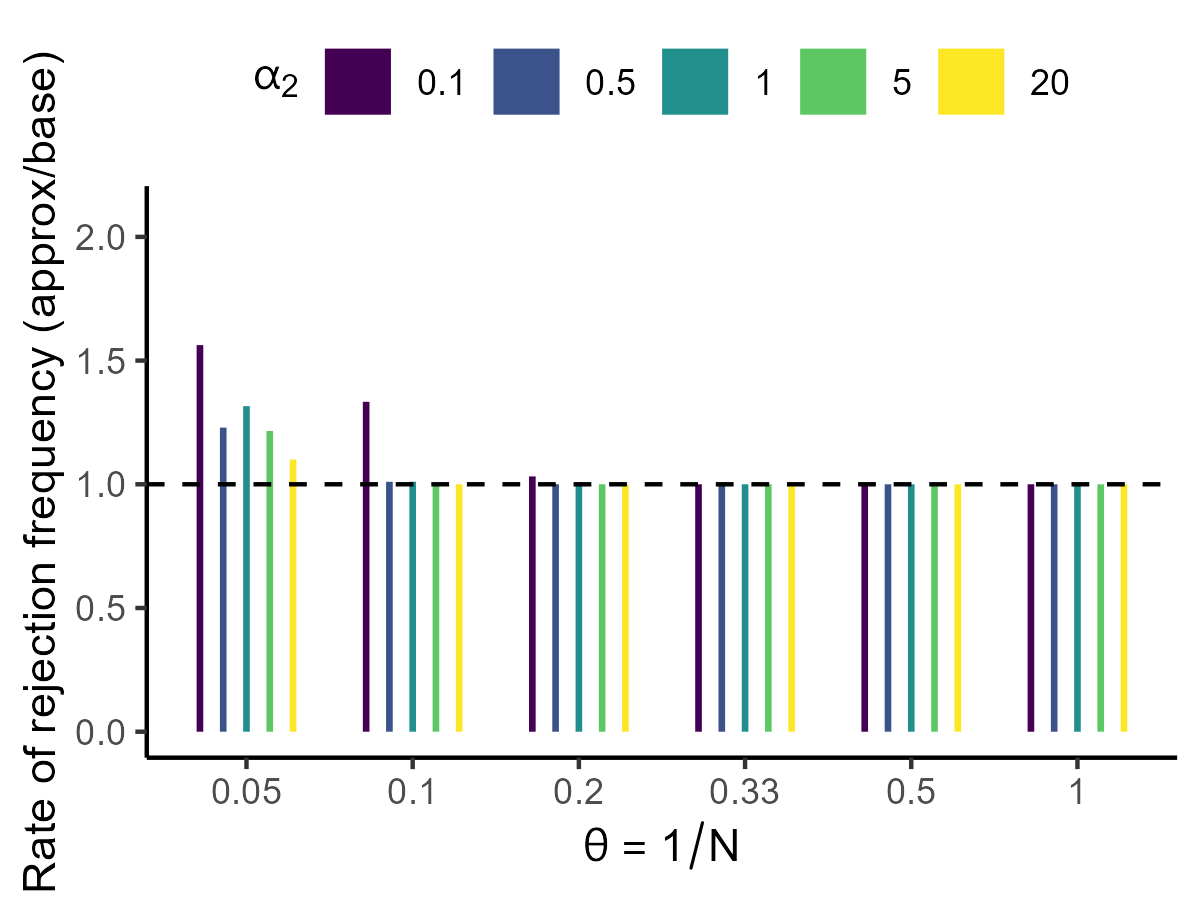
\includegraphics[width = 0.32\textwidth]
  {figuretable/theta_hat_power_iv_optimal_relative_to_benchmark_10000.png}}
  \caption{Relative efficiency gain of optimal instruments}
  \label{fg:theta_hat_power_iv_optimal_relative_to_benchmark_10000}
  \end{center}
\end{figure} 



\section{Conclusion}

We perform a statistical power analysis for conduct parameter estimation. Power rises with an increase in the number of markets, a larger conduct parameter, and a stronger demand rotation instrument. 
Nevertheless, rejecting the null hypothesis of markets operating under perfect competition remains challenging, even with a moderate number of markets (e.g., 1000) and five firms, regardless of instrument strength and the use of optimal instruments. 
This reaffirms that the difficulty in testing perfect competition, as observed by \cite{genesove1998testing}, \cite{steen1999testing}, and \cite{shaffer1993test}, is primarily attributed to the limited number of markets, rather than methodological shortcomings.

\paragraph{Acknowledgments}
We thank Jeremy Fox, Isabelle Perrigne, and Yuya Shimizu for their valuable advice. This research did not receive any specific grant from funding agencies in the public, commercial, or not-for-profit sectors. 

\newpage


\bibliographystyle{aer}
\bibliography{conduct_parameter}

\newpage

\setcounter{page}{1}
\appendix
\section{Online appendix}\label{sec:appendix}




\subsection{Details for our simulation settings}

To generate the simulation data, for each model, we first generate the exogenous variables $Y_{t}, Z^{R}_{t}, W_{t}, R_{t}, H_{t}$, and $K_{t}$ and the error terms $\varepsilon_{t}^c$ and $\varepsilon_{t}^d$ based on the data generation process in Table \ref{tb:parameter_setting}.
We compute the equilibrium quantity $Q_{t}$ for the linear model by \eqref{eq:quantity_linear}.
We then compute the equilibrium price $P_{t}$ by substituting $Q_{t}$ and other variables into the demand function \eqref{eq:linear_demand}.

We estimate the equations using the \texttt{ivreg} package in \texttt{R}.
An important feature of the model is that we have an interaction term of the endogenous variable $Q_{t}$ and the instrumental variable $Z^{R}_{t}$.
The \texttt{ivreg} package automatically detects that the endogenous variables are $Q_{t}$ and the interaction term $Z^{R}_{t}Q_{t}$, running the first stage regression for each endogenous variable with the same instruments. To confirm this, we manually write R code to implement the 2SLS model. 
When the first stage includes only the regression of $Q_{t}$, estimation results from our code differ from the results from \texttt{ivreg}. 
However, when we modify the code to regress $Z^{R}_{t}Q_{t}$ on the instrument variables and estimate the second stage by using the predicted values of $Q_{t}$ and $Z^{R}_{t}Q_{t}$, the result from our code and the result from \texttt{ivreg} coincide.

% \subsubsection{GMM}


% In the first step, solve the minimization problem with a weight matrix $\Omega = (Z^\top Z)^{-1}/T$.
% Then compute the optimal instrument based on the estimation result in the first step.
% In the second step, replace the instrument variables with the optimal instrument and solve the minimization problem.


\subsection{Optimal instruments}\label{sec:optimal_instruments}
We begin by introducing optimal instruments for a simultaneous equation model. Subsequently, we move to supply-side estimation, as the simultaneous equation model does not yield any additional efficiency advantage when the error terms in the demand and supply equations are uncorrelated, as in our scenario.

We define demand and supply residuals as follows.
\begin{align*}
    \varepsilon^{d}_{t}(\xi) &= P_{t} - \alpha_0 + (\alpha_1 + \alpha_2Z^{R}_{t})Q_{t} - \alpha_3 Y_{t},\\
    \varepsilon^c_{t}(\xi) &= P_{t} - \gamma_0 - \theta (\alpha_1 + \alpha_2 Z^{R}_{t})Q_{t} - \gamma_1 Q_{t} - \gamma_2 W_{t} - \gamma_3 R_{t},
\end{align*}
where $\xi=\left(\alpha_0, \alpha_1, \alpha_2, \alpha_3, \gamma_0, \gamma_1, \gamma_2, \gamma_3, \theta\right)$ is the $9\times 1$ parameter vector. 
Let $Z_{t}=(Z_{t}^{d},Z_{t}^{s})$ and $\varepsilon_{t}(\xi)=(\varepsilon_{t}^{d}(\xi),\varepsilon_{t}^{s}(\xi))'$.
We make the assumption that $\Omega=E[\varepsilon_{t}\varepsilon_{t}'|Z_{t}]$ is a constant $2\times 2$ matrix, defining the covariance structure of the demand and supply residuals.
The optimal instrument matrix of \cite{chamberlain1987asymptotic} is the $9\times 2$ matrix $g_{t}(Z_{t})=D_{t}(Z_{t})'\Omega^{-1}$
where the $2\times 9$ matrix $D_{t}(Z_{t})=E\left[\frac{\partial \varepsilon_{t}}{\partial \xi}| Z_{t}\right]$ is the conditional expectation of the derivative of the conditional moment restrictions with respect to parameters $\xi$. 

The conditional expectation $D_{t}(Z_{t})$ is difficult to compute, so most applications have considered approximations. As in \cite{reynaert2014improving}, we consider two types of approximation. 
The first approximation for $D_{t}(Z_{t})$ takes a second-order polynomial of $Z_{t}$ for the demand side instruments (first row of $D_{t}(Z_{t})$), i.e. cost shifters $W_{t}$ and $R_{t}$, and their squares and interactions, and $W_{t}$ and $R_{t}$ for the supply side instruments (second row of $D_{t}(Z_{t})$).
The second approximation for $D_{t}(Z_{t})$ implements the conditional expectation written as 
\begin{align*}
    &D_{t}(Z_{t})\\
    &=E\left[\frac{\partial \varepsilon_{t}}{\partial \xi}| Z_{t}\right]\\
    &=
    \begin{pmatrix}
    & E\left[\frac{\partial \varepsilon_{t}^{d}(\xi)}{\partial \alpha^{\prime}} \mid Z_{t}\right] & 
    E\left[\frac{\partial \varepsilon_{t}^{d}(\xi)}{\partial \gamma^{\prime}} \mid Z_{t}\right] & 
    E\left[\frac{\partial \varepsilon_{t}^{d}(\xi)}{\partial \theta} \mid Z_{t}\right]\\
    & E\left[\frac{\partial \varepsilon_{t}^{c}(\xi)}{\partial \alpha^{\prime}} \mid Z_{t}\right] & 
    E\left[\frac{\partial \varepsilon_{t}^{c}(\xi)}{\partial \gamma^{\prime}} \mid Z_{t}\right] & 
    E\left[\frac{\partial \varepsilon_{t}^{c}(\xi)}{\partial \theta} \mid Z_{t}\right]
    \end{pmatrix} \\
    &=\begin{pmatrix}
    -1 & 
    \overline{Q}_{t} & 
    Z^{R} \overline{Q}_{t} & 
    - Y_{t} &
    0 & 0 & 0 & 0 & 0 \\
    0 &- \theta \overline{Q}_{t} & -\theta Z^{R}_{t}\overline{Q}_{t} & 0 & 
    -1 &
    - \overline{Q}_{t} &
    -W_{t} &
    -R_{t} &
    -(\alpha_1 + \alpha_2 Z^{R}_{t})\overline{Q}_{t}
    \end{pmatrix},
\end{align*}
where $ \overline{Q}_{t} \equiv E[Q_{t}\mid Z_{t}]$. Following the literature, we replace $ \overline{Q}_{t}$ with the fitted values of regressions of $Q_{t}$ on the second order polynomials of $(Y_{t}, Z_{t}^{R}, W_{t}, R_{t}, H_{t}, K_{t})$ and the interactions.

% \textcolor{blue}{
% In our model, $E[Q_{t}\mid Z_{t}]$ can be explicitly obtained because $E[\varepsilon_{t}^{d}\mid Z_{t}^{R}] = E[\varepsilon_{t}^{c}\mid Z_{t}^{R}] = 0 $:
% \begin{align*}
%     E[Q_{t}\mid Z_{t}] &=E\left[\left.\frac{\alpha_0 + \alpha_3 Y_{t} - \gamma_0 - \gamma_2 W_{t} - \gamma_3 R_{t} + \varepsilon^{d}_{t} - \varepsilon^{c}_{t}}{(1 + \theta) (\alpha_1 + \alpha_2 Z^{R}_{t}) + \gamma_1}\right| Z_{t}\right] \\
%     & = \frac{\alpha_0 + \alpha_3 Y_{t} - \gamma_0 - \gamma_2 W_{t} - \gamma_3 R_{t}}{(1 + \theta) (\alpha_1 + \alpha_2 Z^{R}_{t}) + \gamma_1},\\
%     E[Z^{R}_{t}Q_{t}\mid Z_{t}] &=E\left[\left. Z^{R}_{t}\frac{\alpha_0 + \alpha_3 Y_{t} - \gamma_0 - \gamma_2 W_{t} - \gamma_3 R_{t} + \varepsilon^{d}_{t} - \varepsilon^{c}_{t}}{(1 + \theta) (\alpha_1 + \alpha_2 Z^{R}_{t}) + \gamma_1}\right | Z_{t}\right]\\
%     & = Z^{R}_{t}\frac{\alpha_0 + \alpha_3 Y_{t} - \gamma_0 - \gamma_2 W_{t} - \gamma_3 R_{t}}{(1 + \theta) (\alpha_1 + \alpha_2 Z^{R}_{t}) + \gamma_1},\\
%     E[(\alpha_1 + \alpha_2 Z^{R}_{t})Q_{t}\mid Z_{t}] &=E\left[\left. (\alpha_1 + \alpha_2 Z^{R}_{t})\frac{\alpha_0 + \alpha_3 Y_{t} - \gamma_0 - \gamma_2 W_{t} - \gamma_3 R_{t}}{(1 + \theta) (\alpha_1 + \alpha_2 Z^{R}_{t}) + \gamma_1}\right | Z_{t}\right]\\
%     &= (\alpha_1 + \alpha_2 Z^{R}_{t})\frac{\alpha_0 + \alpha_3 Y_{t} - \gamma_0 - \gamma_2 W_{t} - \gamma_3 R_{t}}{(1 + \theta) (\alpha_1 + \alpha_2 Z^{R}_{t}) + \gamma_1}.
% \end{align*}
% }
When only the supply side is estimated given fixed demand parameters as in our main results, the earlier optimal instrument matrix is modified into the $5\times 1$ matrix $g_{t}(Z_{t})=D_{t}(Z_{t})'$ where 
\begin{align*}
    D_{t}(Z_{t}) &= \begin{pmatrix}
     & 
    E\left[\frac{\partial \varepsilon_{t}^{c}(\xi)}{\partial \gamma^{\prime}} \mid Z_{t}\right] & 
    E\left[\frac{\partial \varepsilon_{t}^{c}(\xi)}{\partial \theta} \mid Z_{t}\right]
    \end{pmatrix} \\
    &=\begin{pmatrix}
    -1 &
    -\overline{Q}_{t} &
    -W_{t} &
    -R_{t} &
    -(\alpha_1 + \alpha_2 Z^{R}_{t})\overline{Q}_{t}
    \end{pmatrix}.
\end{align*}
This suggests augmenting the benchmark instruments with $\overline{Q}_{t}$ and $(\alpha_1 + \alpha_2 Z^{R}{t})\overline{Q}_{t}$.
To prevent redundancy, we add $\overline{Q}_{t}$ to the benchmark model.
We verify that including $(\alpha_1 + \alpha_2 Z^{R}{t})\overline{Q}_{t}$ in addition to $\overline{Q}_{t}$ does not enhance statistical power.



% Given this optimal instrument matrix, we estimate GMM estimator $\xi^{*}$ based on the following minimization
% problem
% \begin{align*}
%     \min \varepsilon'(\xi)g(\xi)\Omega g(\xi)'\varepsilon . 
% \end{align*}
% In this case, $\Omega$ is replaced by the identity matrix.


Figure \ref{fg:theta_hat_power_iv_polynomial_relative_to_benchmark} reports the relative efficiency gain of the first approximation approach. 
The efficiency gain is ignorable.
Figure \ref{fg:theta_hat_power_iv_optimal_relative_to_benchmark_10000} in the main text reports the relative efficiency gain of the optimal instruments in the second approach. 
The efficiency gain is significant when the number of markets is more than 1,000. 
However, this does not change our benchmark results.


\begin{figure}[!ht]
  \begin{center}
  % \subfloat[M=50]{\includegraphics[width = 0.32\textwidth]
  % {figuretable/theta_hat_power_50.png}}
  \subfloat[$T=100$]{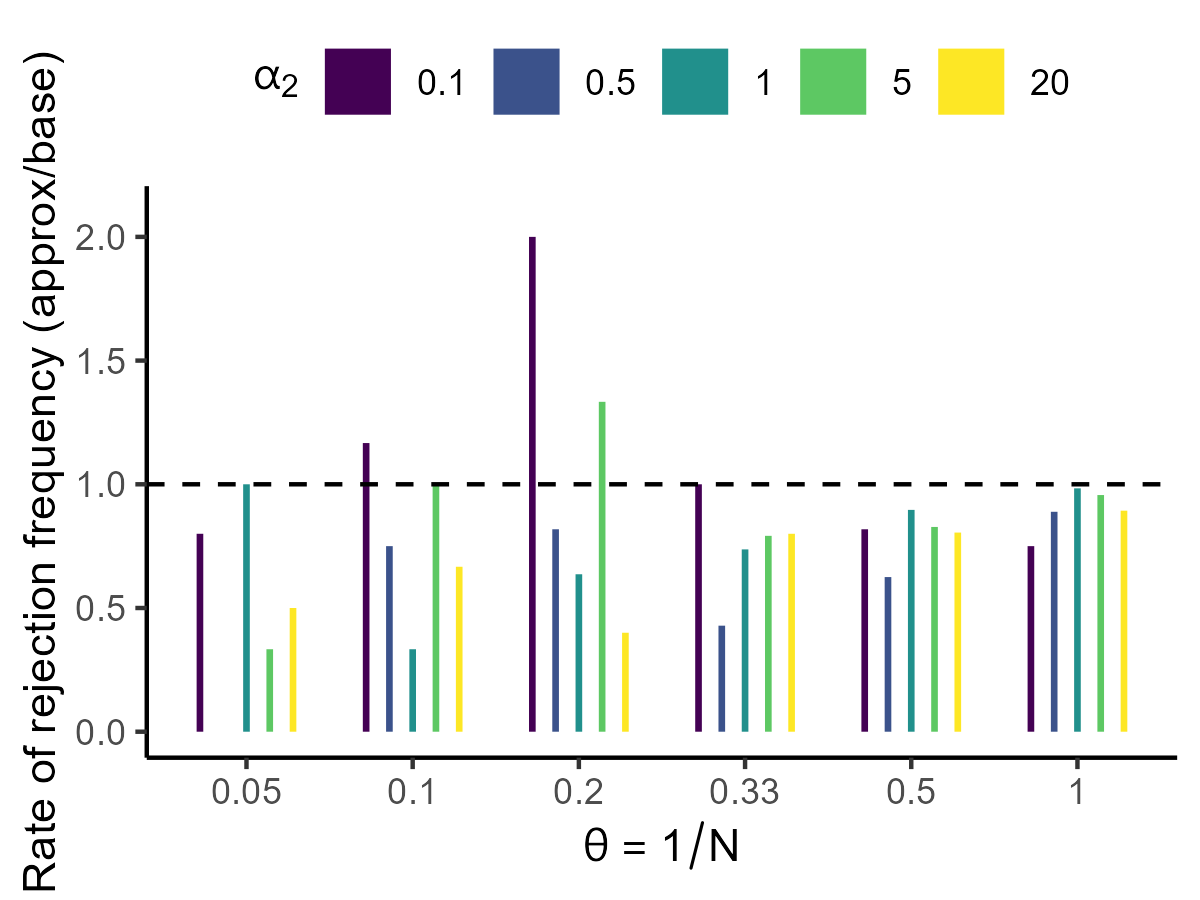
\includegraphics[width = 0.32\textwidth]
  {figuretable/theta_hat_power_iv_polynomial_relative_to_benchmark_100.png}}
  \subfloat[$T=200$]{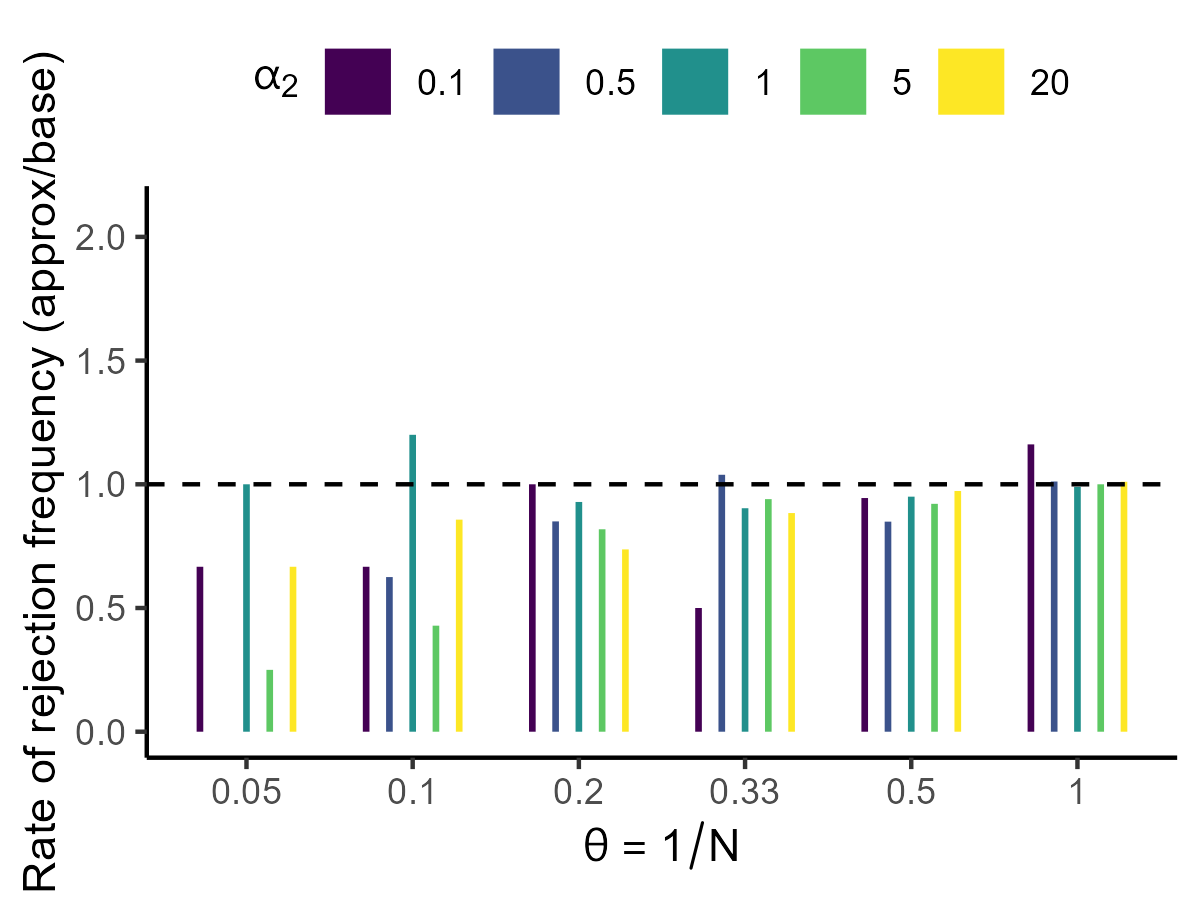
\includegraphics[width = 0.32\textwidth]
  {figuretable/theta_hat_power_iv_polynomial_relative_to_benchmark_200.png}}
  \subfloat[$T=1000$]{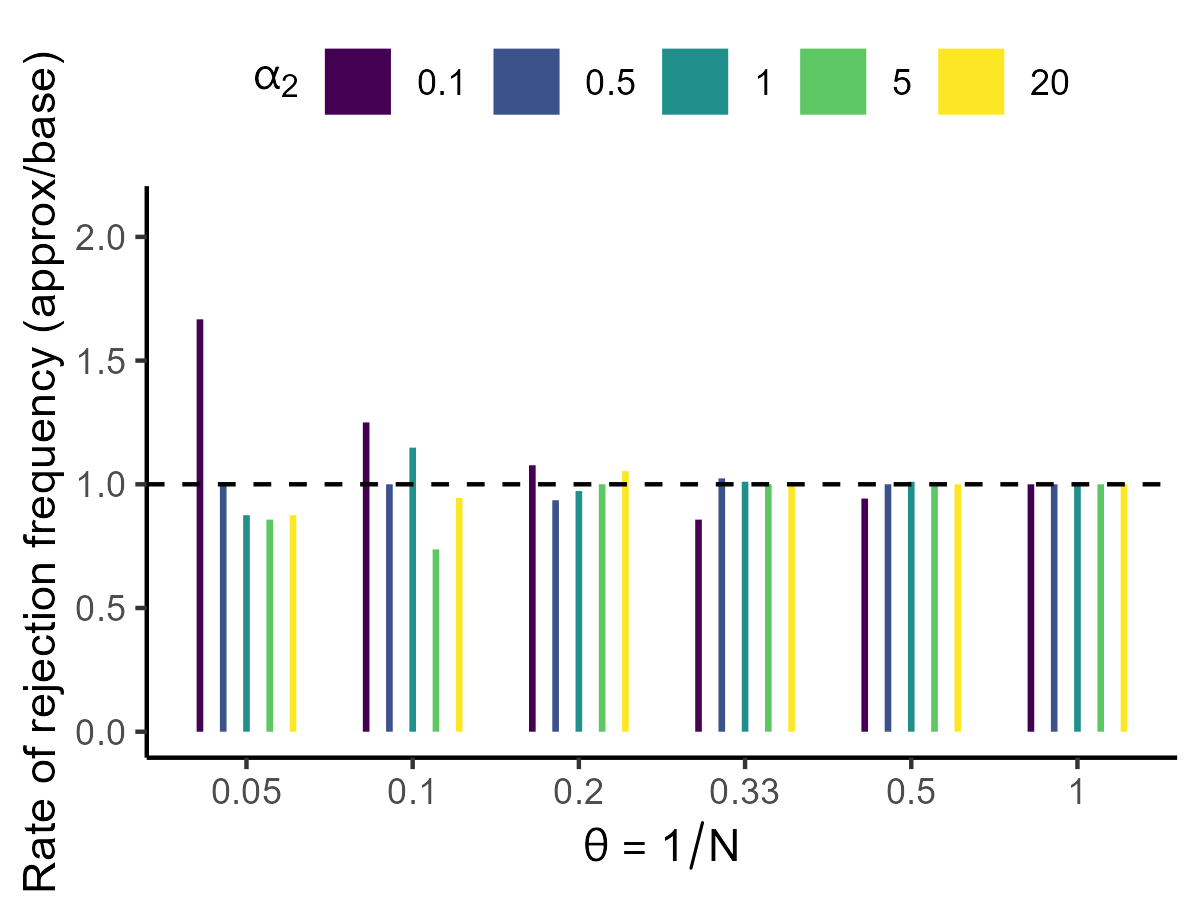
\includegraphics[width = 0.32\textwidth]
  {figuretable/theta_hat_power_iv_polynomial_relative_to_benchmark_1000.png}}\\
  \subfloat[$T=2000$]{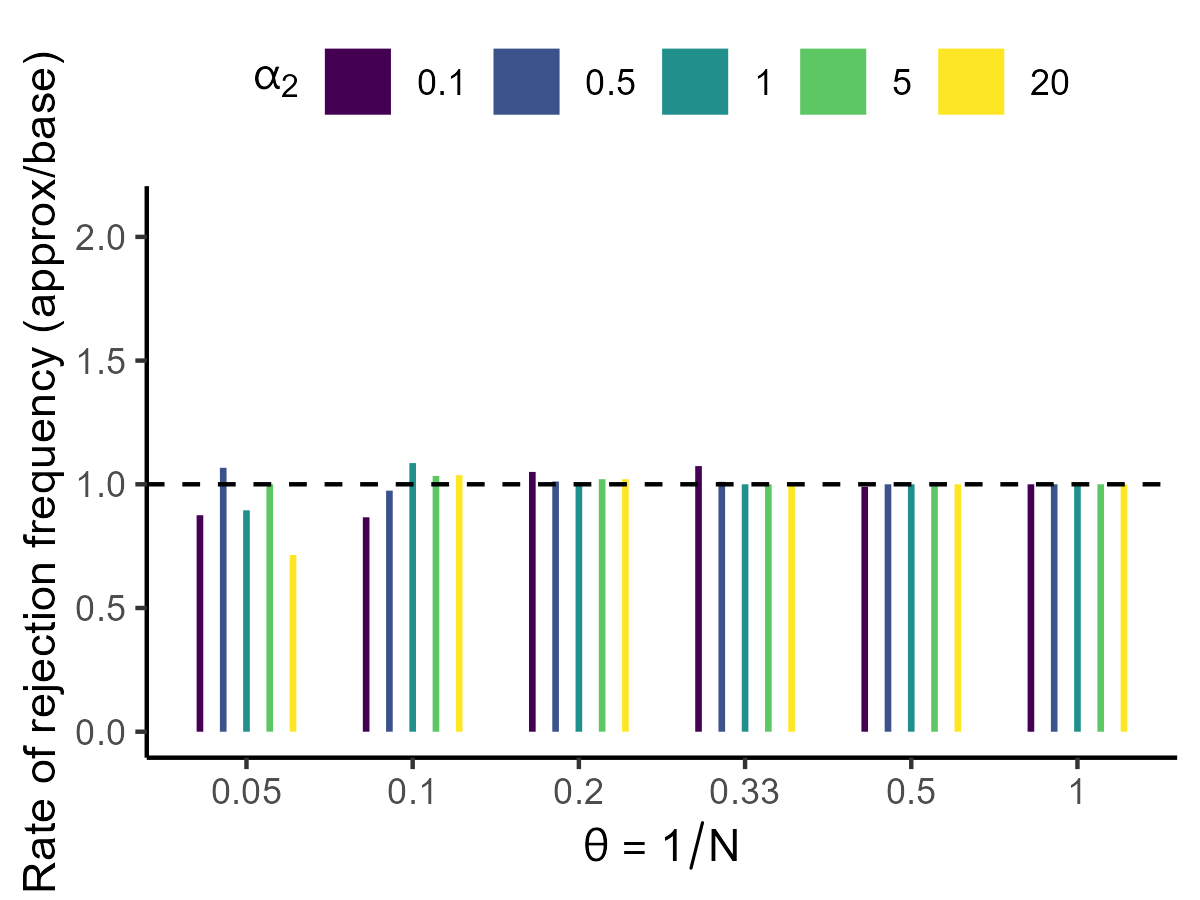
\includegraphics[width = 0.32\textwidth]
  {figuretable/theta_hat_power_iv_polynomial_relative_to_benchmark_2000.png}}
  \subfloat[$T=5000$]{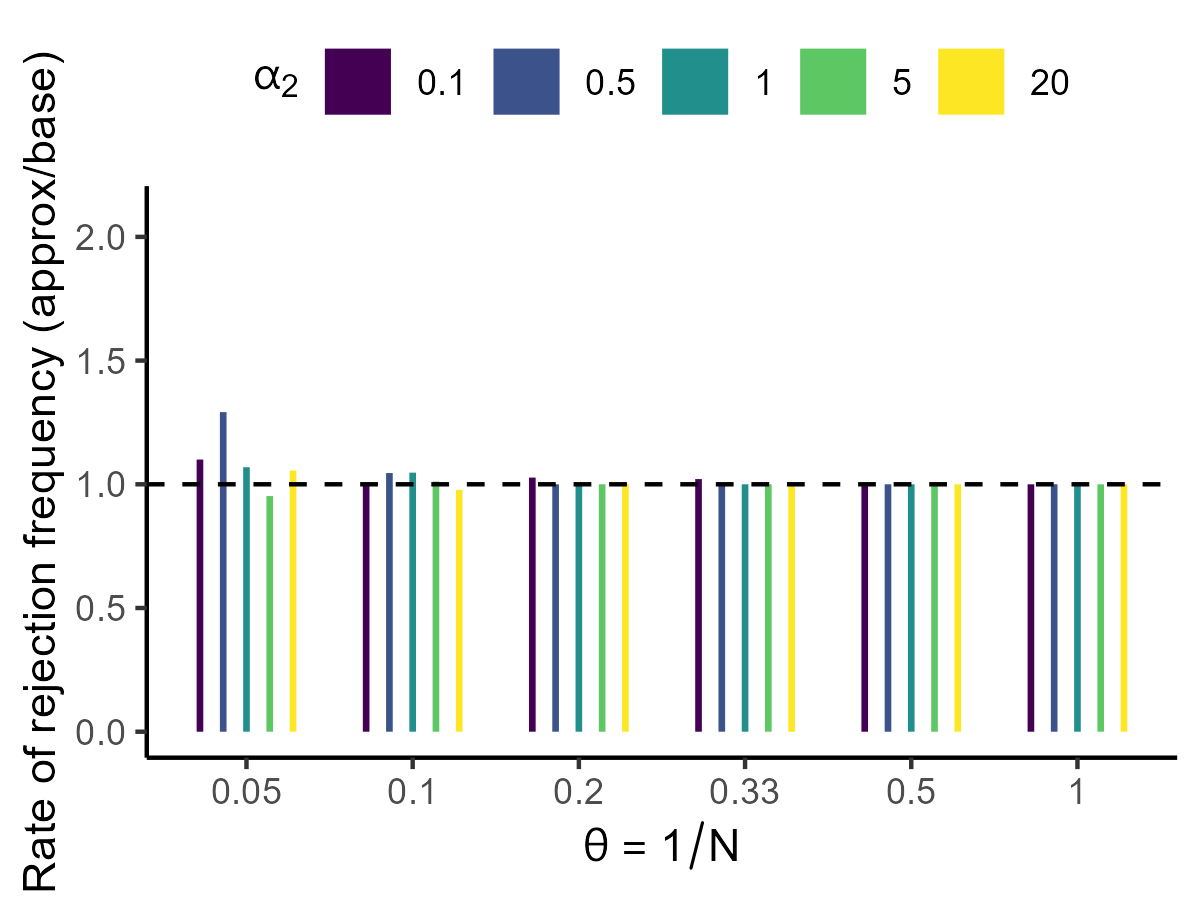
\includegraphics[width = 0.32\textwidth]
  {figuretable/theta_hat_power_iv_polynomial_relative_to_benchmark_5000.png}}
  \subfloat[$T=10000$]{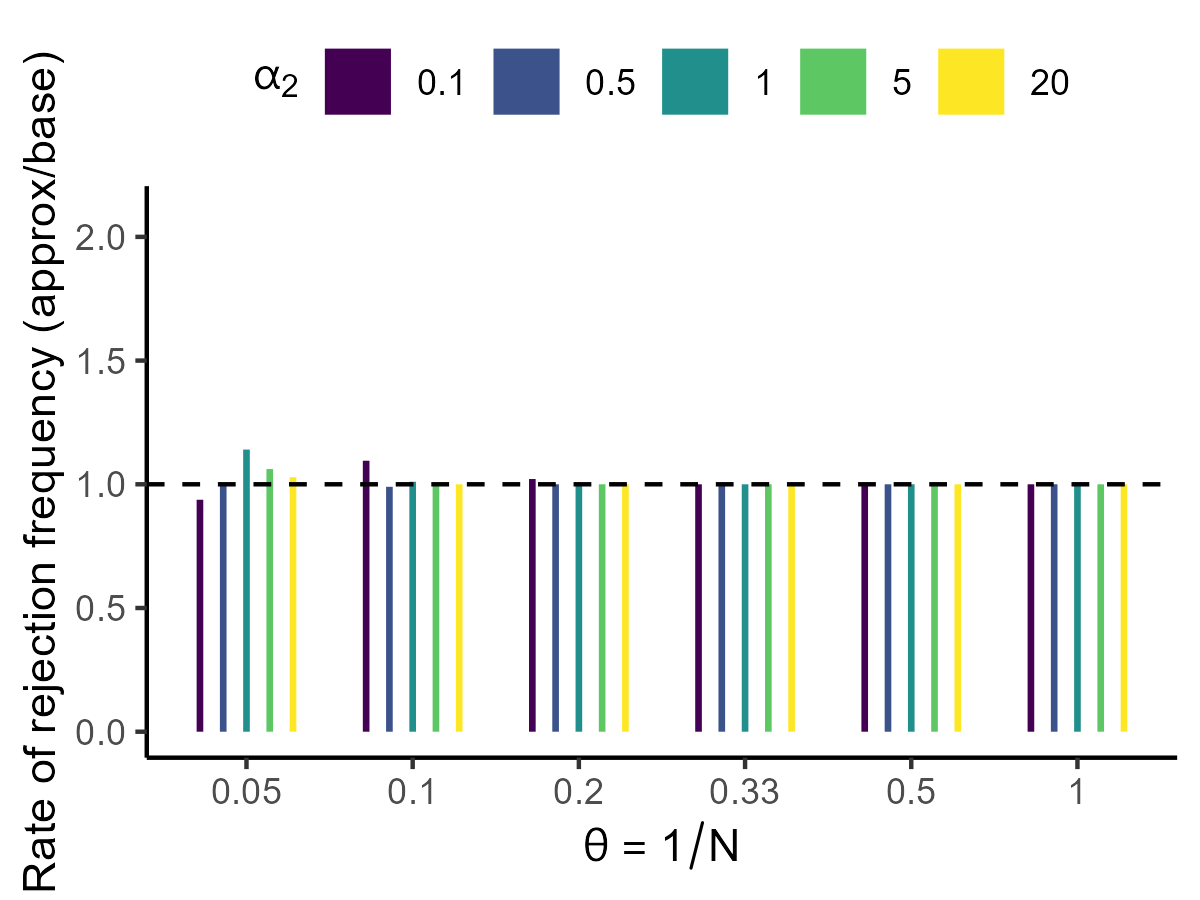
\includegraphics[width = 0.32\textwidth]
  {figuretable/theta_hat_power_iv_polynomial_relative_to_benchmark_10000.png}}
  \caption{Relative efficiency gain of the first approximation approach}
  \label{fg:theta_hat_power_iv_polynomial_relative_to_benchmark}
  \end{center}
  % \footnotesize
  % Note: Dotted lines are 80\% and 100\% rejection frequencies out of 100 simulation data.
\end{figure} 


% \subsection{Optimal IV separate}

% \begin{figure}[!ht]
%   \begin{center}
%   % \subfloat[M=50]{\includegraphics[width = 0.32\textwidth]
%   % {figuretable/theta_hat_power_50.png}}
%   \subfloat[$T=100$]{\includegraphics[width = 0.32\textwidth]
%   {figuretable/theta_hat_power_iv_optimal_separate_relative_to_benchmark_100.png}}
%   \subfloat[$T=200$]{\includegraphics[width = 0.32\textwidth]
%   {figuretable/theta_hat_power_iv_optimal_separate_relative_to_benchmark_200.png}}
%   \subfloat[$T=1000$]{\includegraphics[width = 0.32\textwidth]
%   {figuretable/theta_hat_power_iv_optimal_separate_relative_to_benchmark_1000.png}}\\
%   \subfloat[$T=2000$]{\includegraphics[width = 0.32\textwidth]
%   {figuretable/theta_hat_power_iv_optimal_separate_relative_to_benchmark_2000.png}}
%   \subfloat[$T=5000$]{\includegraphics[width = 0.32\textwidth]
%   {figuretable/theta_hat_power_iv_optimal_separate_relative_to_benchmark_5000.png}}
%   \subfloat[$T=10000$]{\includegraphics[width = 0.32\textwidth]
%   {figuretable/theta_hat_power_iv_optimal_separate_relative_to_benchmark_10000.png}}
%   \caption{Rate of statistical power of conduct parameter $\theta$: Separate}
%   \label{fg:theta_hat_power_iv_polynomial_relative_to_benchmark}
%   \end{center}
%   % \footnotesize
%   % Note: Dotted lines are 80\% and 100\% rejection frequencies out of 100 simulation data.
% \end{figure} 


% \begin{figure}[!ht]
%   \begin{center}
%   % \subfloat[M=50]{\includegraphics[width = 0.32\textwidth]
%   % {figuretable/theta_hat_power_50.png}}
%   \subfloat[$T=100$]{\includegraphics[width = 0.32\textwidth]
%   {figuretable/theta_hat_power_separate_100.png}}
%   \subfloat[$T=200$]{\includegraphics[width = 0.32\textwidth]
%   {figuretable/theta_hat_power_separate_200.png}}
%   \subfloat[$T=1000$]{\includegraphics[width = 0.32\textwidth]
%   {figuretable/theta_hat_power_separate_1000.png}}\\
%   \subfloat[$T=2000$]{\includegraphics[width = 0.32\textwidth]
%   {figuretable/theta_hat_power_separate_2000.png}}
%   \subfloat[$T=5000$]{\includegraphics[width = 0.32\textwidth]
%   {figuretable/theta_hat_power_separate_5000.png}}
%   \subfloat[$T=10000$]{\includegraphics[width = 0.32\textwidth]
%   {figuretable/theta_hat_power_separate_10000.png}}
%   \caption{Statistical power of conduct parameter $\theta$: Separate}
%   \label{fg:theta_hat_power}
%   \end{center}
%   \footnotesize
%   Note: Dotted lines are 80\% and 100\% rejection frequencies out of 100 simulation data.
% \end{figure} 


\subsection{Additional results}
Estimation results of all parameters except conduct parameter $\theta$ are shown on the author's github. 
Totally, we confirm that estimation is accurate with small bias and root-mean-squared error when increasing sample size, as in \cite{matsumura2023resolving}.
Interested readers can modify the current data-generating process.



\end{document}